% !TEX root = msc_thesis.tex

\chapter{Results} \label{chap:results}

After making all the changes described in the implementation, we retrained the core and interface predictors and validated them on new data.


ELASPIC uses the gradient boosting of decision trees regressor (GBR). It was optimized in several ways.

ELASPIC described in  output xxx features in total.
1. We calculated those features for the Provean and the Skempi training sets.
2. We removed features that were note different in any of the training cases (xxx for core mutations and yyy for interface mutations).

3. It has been reported that balancing the training set by including both positive and negative samples


As described in [], balancing the training set can significantly improve performance. However, with Provean balancing the training set can bias the result because most mutations are to unconserved amino acids (often alanine) and



We built two core predictors and two interface predictors:

\begin{enumerate}
	\item No sequence features but a balanced training set.
	\item Sequence features but no balanced training set.
\end{enumerate}

- Accuracy over different sequence identity bins

- within protein correlation on the test set



\section{Datasets}

\begin{table}[!htb]
	\caption[Datasets used in this study.]{Description of the datasets that were used in this study.}
	\label{tab:datasets}
	\begin{tabular}{ l |  p{1.8cm} | p{9cm} }
		\toprule
		Name                  & Type               & Description                                                                                                                                                                                                                                                                                                                  \\
		\midrule
		\textbf{Protherm}     & Train              & Database of mutations-induced changes in the Gibbs free energy of protein folding ($\Delta \Delta G_{core}$)  \cite{kumar_protherm_2006}.                                                                                                                                                                                    \\
		\textbf{Skempi}       & Train              & Database of mutations-induced changes in the Gibbs free energy of protein-protein interactions ($\Delta \Delta G_{interface}$) \cite{moal_skempi:_2012}.                                                                                                                                                                     \\
		\textbf{Taipale}      & Validation         & Interaction between chaperones and wildtype or mutant proteins, quantified using the LUMIER assay \cite{sahni_widespread_2015}.                                                                                                                                                                                              \\
		\textbf{Taipale PPI}  & Validation         & Results of yeast two-hybrid experiments, measuring the presence or absence of protein-protein interactions for wild-type and mutant proteins \cite{sahni_widespread_2015}.                                                                                                                                                   \\
		\textbf{Taipale GPCA} & Validation         & \textit{Gaussia princeps} luciferase protein complementation assay, measuring the effect of mutations on protein affinity \cite{sahni_widespread_2015}.                                                                                                                                                                      \\
		\textbf{Humsavar}     & Validation \& Test & Disease-causing mutations and polymorphisms obtained from the UniProt \textit{humsavar.txt} file \cite{consortium_uniprot:_2015}. Mutations annotated with at least one disease were assigned a value of $1$. Mutations annotated as ``polymorphisms'' were assigned a value of $0$.                                         \\
		\textbf{ClinVar}      & Validation \& Test & Disease-causing mutations and polymorphisms obtained from ClinVar \cite{landrum_clinvar:_2016}. Mutations found in the ClinVar \textit{clinvar\_20160531.vcf} file were assigned a value of $1$. Mutations found in the ClinVar \textit{common\_no\_known\_medical\_impact\_20160531.vcf} file were assigned a value of $0$. \\
		\textbf{COSMIC}       & Validation \& Test & Mutations found in cancer \cite{forbes_cosmic:_2015}. Mutations classified by FATHMM \cite{shihab_ranking_2014} as cancer drivers were assigned a value of $1$. Mutations classified by FATHMM as cancer passengers were assigned a value of $0$.                                                                            \\
		\textbf{SUMO Ligase}  & Test               & Mutations affecting the activity of SUMO ligase, measured using a cell viability assey \cite{cagi4_sumo_ligase}.                                                                                                                                                                                                             \\
		\textbf{AB-Bind}      & Test               & Mutations explored in antibody affinity maturation experiments \cite{sirin_ab-bind:_2016}.                                                                                                                                                                                                                                   \\
		\textbf{Benedix}      & Test               & Mutations from alanine scanning of the TEM1 ($\beta$-lactamase) -- BLIP ($\beta$-lactamase-inhibitor) interface \cite{benedix_predicting_2009}.                                                                                                                                                                              \\
		\bottomrule
	\end{tabular}
\end{table}


% \begin{figure}[ht!]
% 	\centering
% 	\includegraphics[width=0.65\textwidth]{static/elaspic_training_set/data_statistics/training_set_overlap_data_core.pdf}
% 	\caption[Size and overlap of core and interface datasets.]{Size and overlap of core and interface datasets.}
% \end{figure}



\section{Machine learning}

\begin{table}[!htb]
	\centering
	\caption[GradientBoostingRegressor parameters evaluated through gridsearch.]{GradientBoostingRegressor evaluated through gridsearch.}
	\label{tab:gridsearch_parameters}
	\begin{tabular}{ l | l }
		\toprule
		Parameter name     & Parameter value                \\
		\midrule
		alpha              & 0.99, 0.95, 0.9, 0.8, 0.7, 0.5 \\
		learning\_rate     & 0.1, 0.05, 0.02, 0.01          \\
		loss               & huber                          \\
		max\_depth         & 10, 8, 6, 4                    \\
		max\_features      & 1.0, 0.8, 0.5, 0.3, 0.1,       \\
		min\_samples\_leaf & 29, 21, 17, 13, 9, 5, 3        \\
		n\_estimators      & 2000                           \\
		\bottomrule
	\end{tabular}
\end{table}




\clearpage

\section{Predicting mutation induced change Gibbs free energy of protein folding.}

\subsection{Grid-search and feature elimination}

\subsection{Validation}


\begin{figure}[!htb]
	\centering
	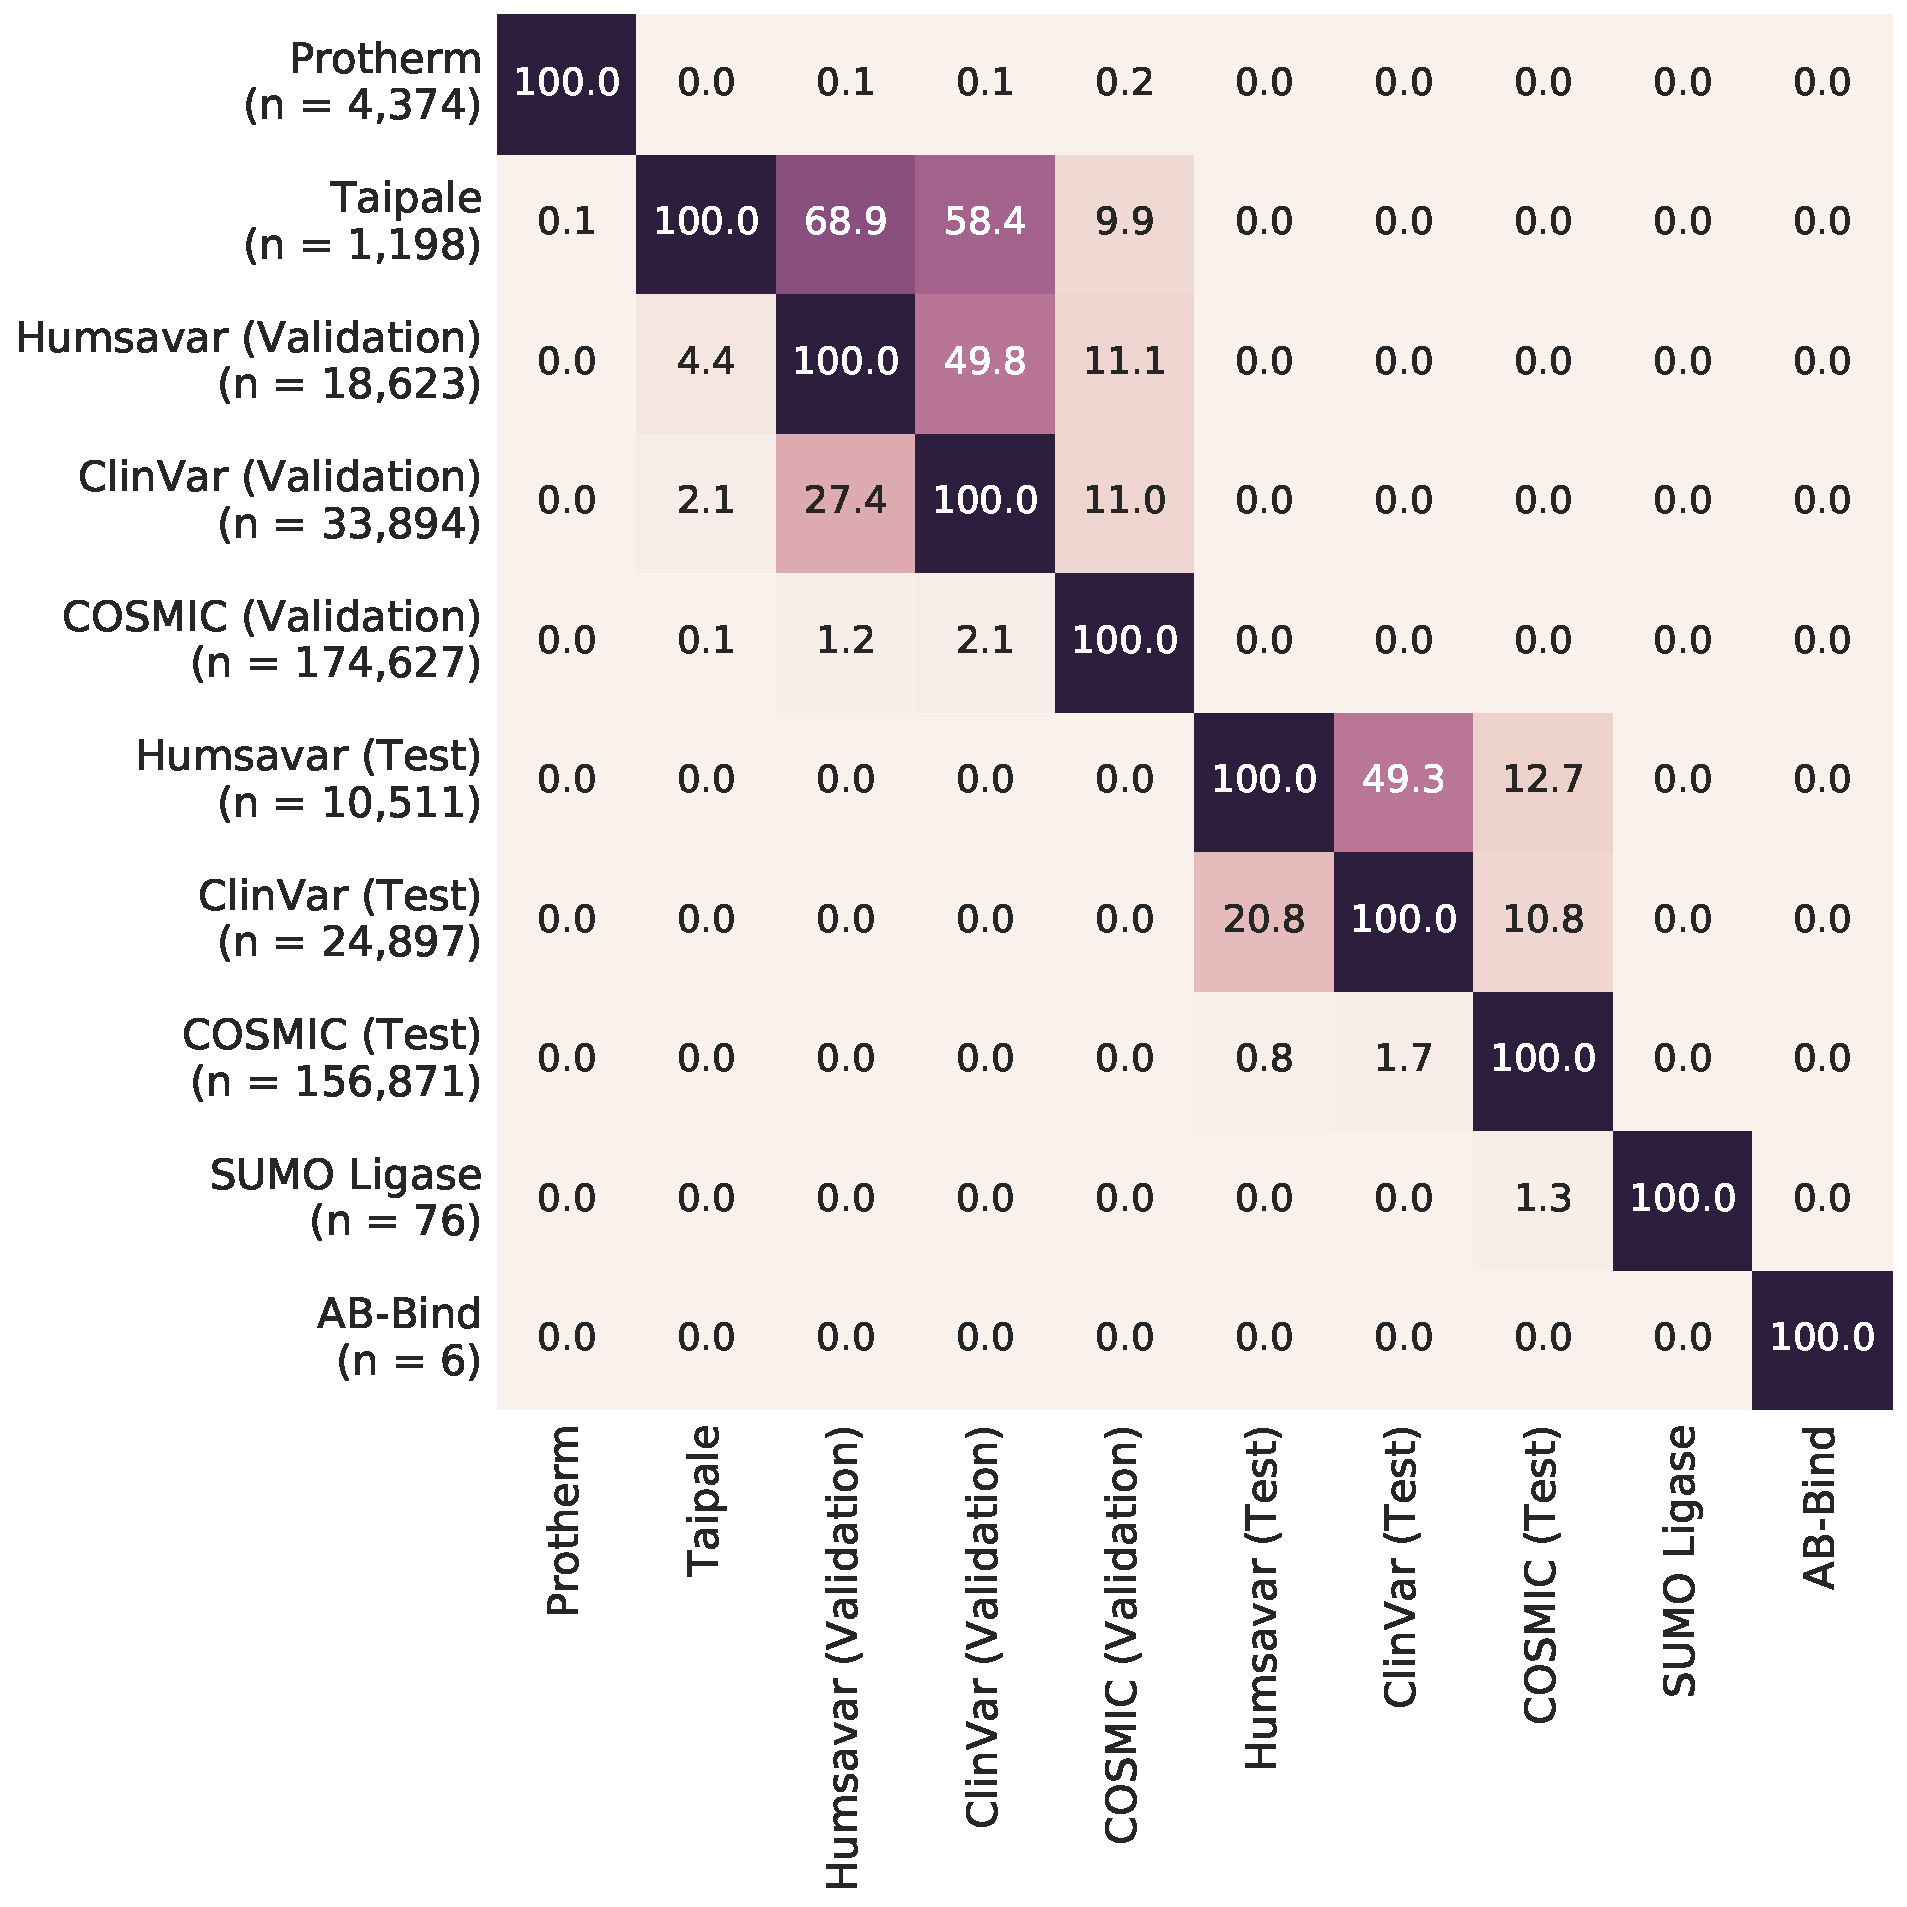
\includegraphics[width=0.8\textwidth]{static/elaspic_training_set/data_statistics/training_set_overlap_data_df_tt_core.pdf}
	\caption[Core predictor datasets.]{Size and overlap of core and interface datasets.}
\end{figure}


% \clearpage
\begin{figure}[!htb]
	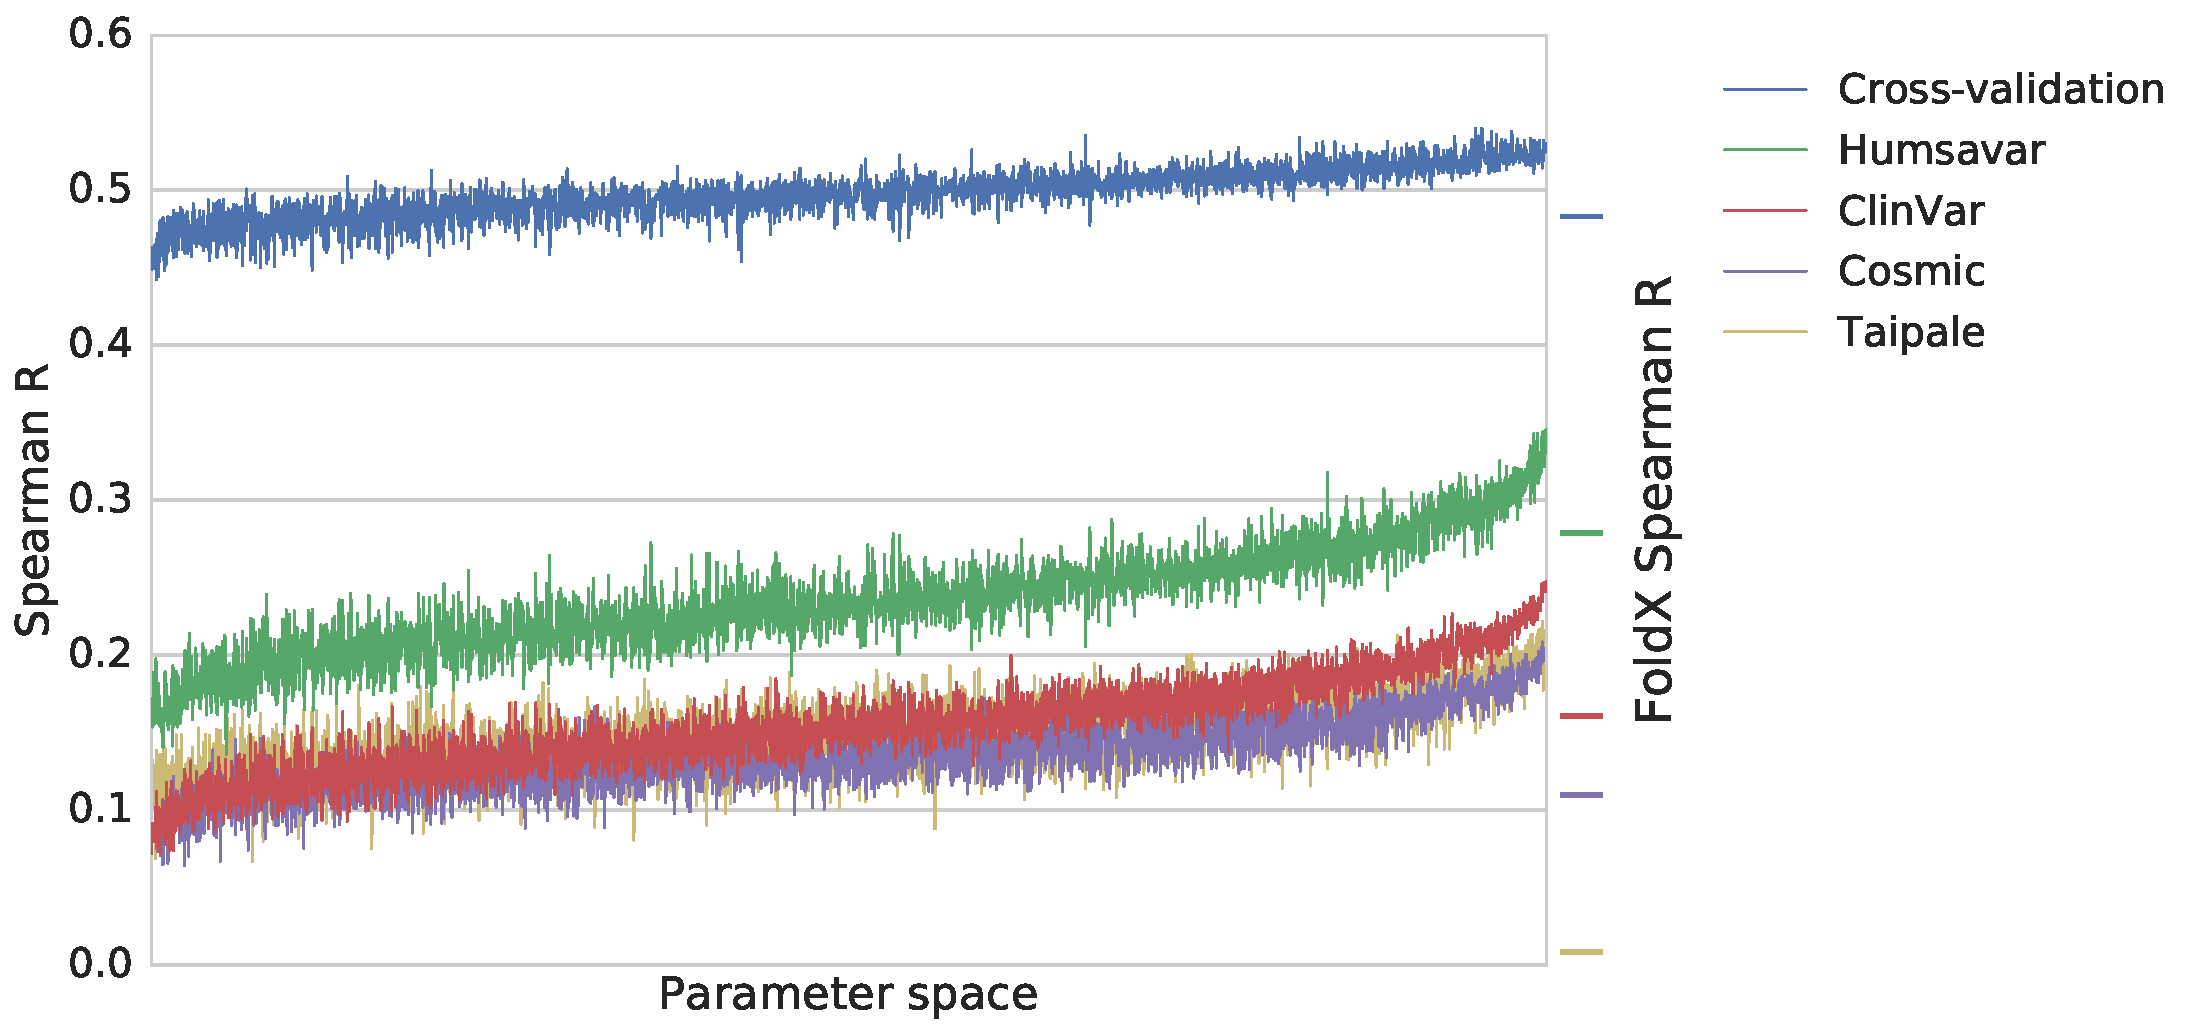
\includegraphics[width=0.9\linewidth]{static/elaspic_training_set/machine_learning/gridsearch_core.pdf}
	\caption{Grid-search over parameter space for the ELASPIC core predictor.}
	\label{fig:gridsearch_core}
\end{figure}


\begin{figure}[!htb]
	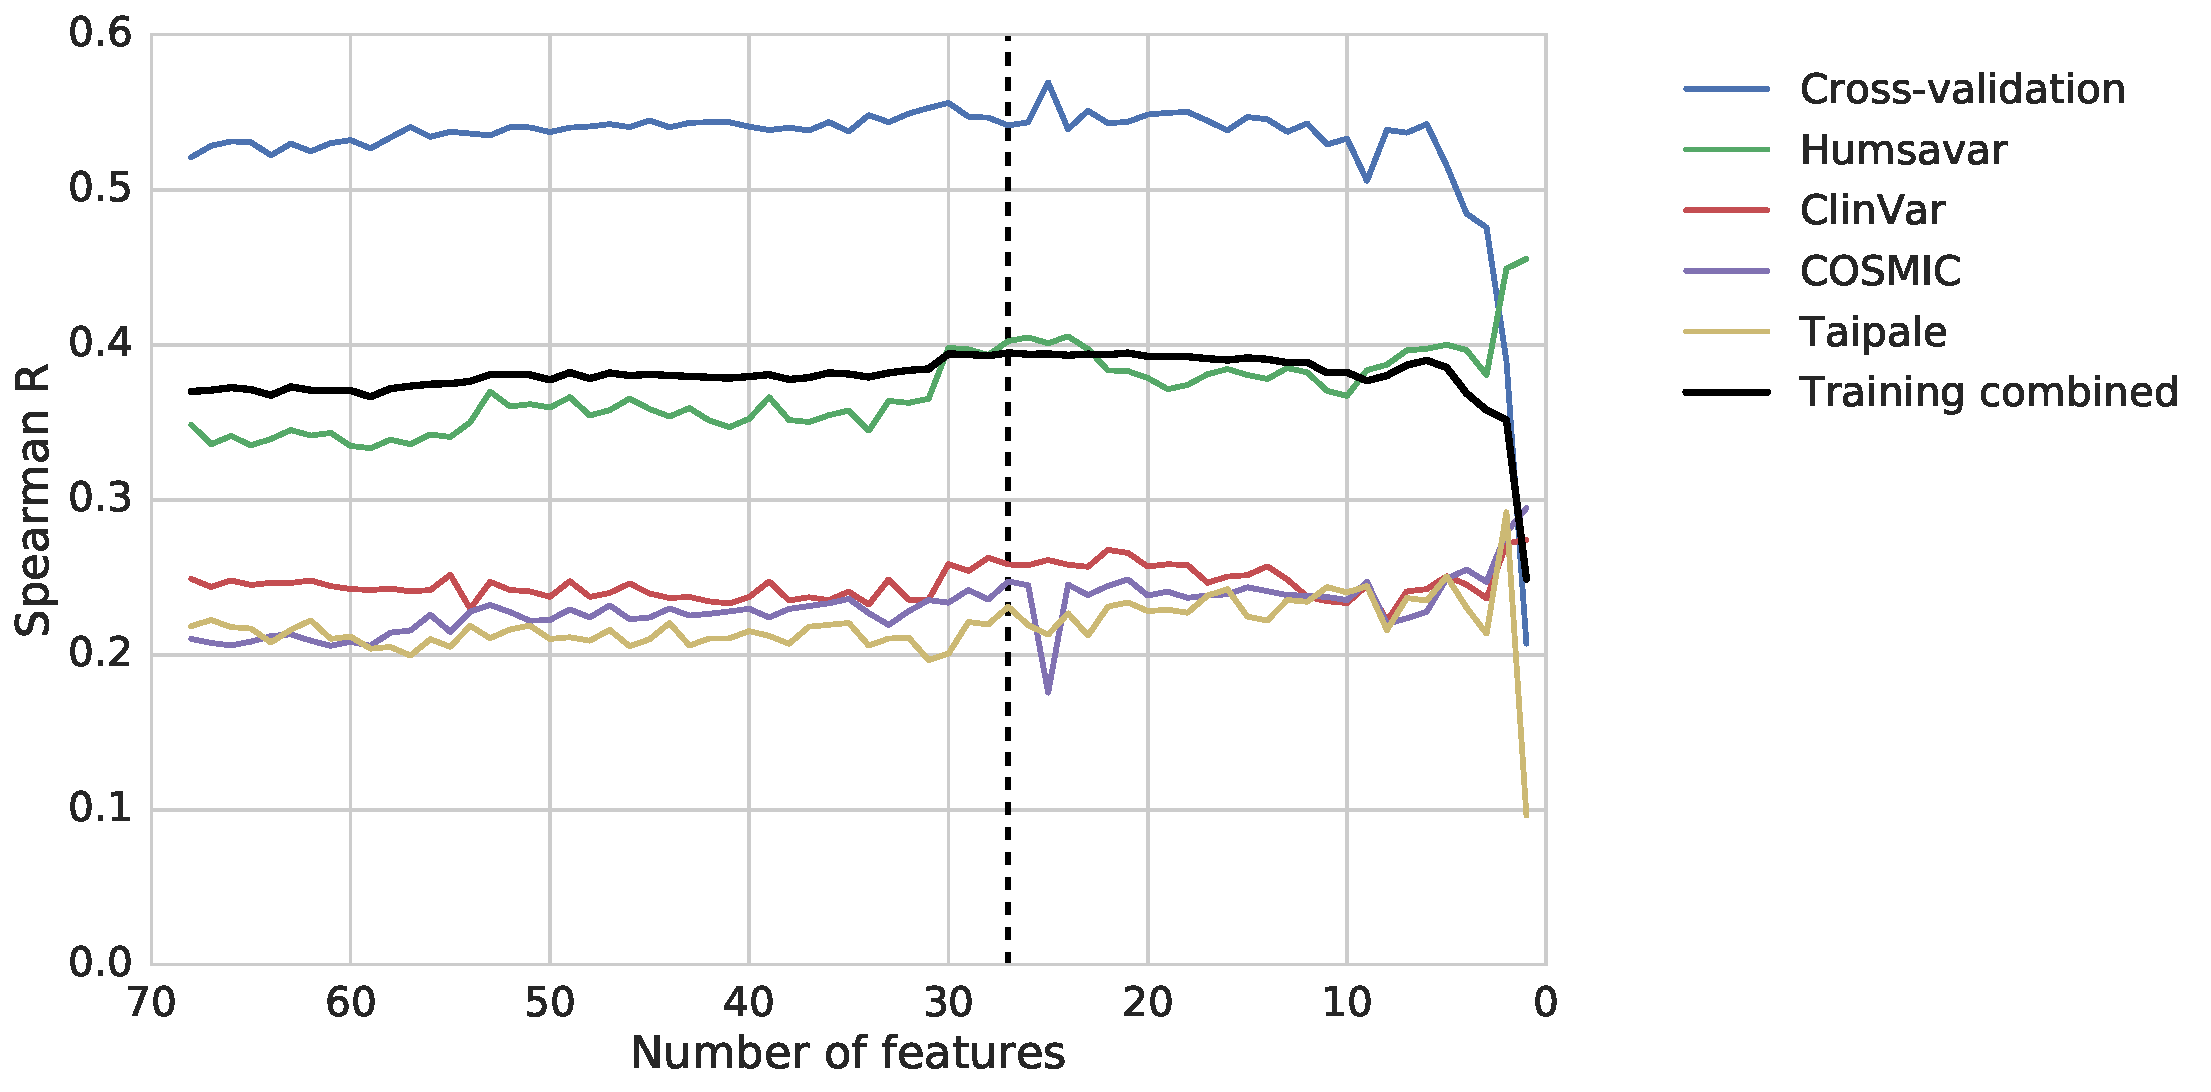
\includegraphics[width=0.9\linewidth]{static/elaspic_training_set/machine_learning/feature_elimination_core.pdf}
	\caption{Feature elimination curve for the ELASPIC core predictor.}
	\label{fig:feature_elimination_core}
\end{figure}


\clearpage
\begin{table}[!htb]
	\centering
	\caption[Core predictor parameters.]{Core predictor parameters.} \label{tab:core_parameters}
	\begin{tabular}{ l | l }
		\toprule
		Parameter name     & Parameter value \\
		\midrule
		alpha              & 0.5             \\
		learning\_rate     & 0.01            \\
		loss               & huber           \\
		max\_depth         & 4               \\
		max\_features      & 0.246           \\
		min\_samples\_leaf & 17              \\
		n\_estimators      & 2000            \\
		\bottomrule
	\end{tabular}
\end{table}


\begin{table}[!htb]
	\centering
	\caption[Core predictor features.]{Core predictor features. Bold indicates the top-6 most important features. FoldX feature descriptions were taken from url{http://foldxsuite.crg.eu/command/Stability}.}
	\label{tab:core_features}
	\begin{tabular}{ l | l | p{7cm} }
		\toprule
		Feature name                              & Feature source & Feature description                                                                                 \\
		\midrule
		alignment\_coverage                       & ELASPIC        & Structural template alignment coverage.                                                             \\
		alignment\_identity                       & ELASPIC        & Structural template sequence identity.                                                              \\
		alignment\_score                          & ELASPIC        & Structural template quality (Equation \ref{eq:core_alignment_score}).                               \\
		backbone\_hbond\_change                   & FoldX          & Backbone hydrogen bond energy.                                                                      \\
		backbone\_hbond\_wt                       & FoldX          & This the contribution of backbone hydrogen bonds.                                                   \\
		cis\_bond\_wt                             & FoldX          & Cis peptide bond energy.                                                                            \\
		disulfide\_wt                             & FoldX          & Contribution of disulfide bonds.                                                                    \\
		electrostatic\_kon\_change                & FoldX          & Electrostatic interaction between molecules in the pre-complex.                                     \\
		\textbf{electrostatics\_change}           & FoldX          & Electrostatic interactions.                                                                         \\
		entropy\_mainchain\_change                & FoldX          & Entropy cost of fixing the main chain.                                                              \\
		helix\_dipole\_wt                         & FoldX          & Electrostatic contribution of the helix dipole.                                                     \\
		matrix\_score                             & ELASPIC        & BLOSUM62 matrix score.                                                                              \\
		pcv\_hbond\_change                        & ELASPIC        & Hydrogen-oxygen contacts involving atoms of the mutated residue and atoms of the interacting chain. \\
		pcv\_hbond\_self\_change                  & ELASPIC        & Hydrogen-oxygen contacts involving atoms of the mutated residue and atoms of the mutated chain.     \\
		pcv\_salt\_equal\_change                  & ELASPIC        & Charge repulsions between atoms of the mutated residue and atoms of the interacting chain.          \\
		pcv\_salt\_equal\_self\_wt                & ELASPIC        & Charge repulsions between atoms of the mutated residue and atoms of the mutated chain.              \\
		pcv\_salt\_equal\_wt                      & ELASPIC        & Charge repulsions between atoms of the mutated residue and atoms of the interacting chain.          \\
		pcv\_salt\_opposite\_change               & ELASPIC        & Charge attractions between atoms of the mutated residue and atoms of the interacting chain.         \\
		pcv\_vdw\_self\_change                    & ELASPIC        & Carbon carbon contacts between atoms of the mutated residue and atoms of the mutated chain.         \\
		\textbf{provean\_score}                   & Provean        & Sequence conservation score.                                                                        \\
		sloop\_entropy\_wt                        & FoldX          & Entropic cost according to the SLoop database of loop conformations.                                \\
		\textbf{solvation\_hydrophobic\_change}   & FoldX          & Contribution of hydrophobic groups.                                                                 \\
		\textbf{solvation\_polar\_change}         & FoldX          & Energetic penalty for burying polar groups.                                                         \\
		\textbf{solvent\_accessibility\_wt}       & MSMS           & Solvent-accessible surface area of the mutated residue.                                             \\
		torsional\_clash\_change                  & FoldX          & Intra-residue Van der Waals torsional clashes.                                                      \\
		\textbf{van\_der\_waals\_clashes\_change} & FoldX          & Energy penalization due to Van der Waals clashes (interresidue).                                    \\
		water\_bridge\_wt                         & FoldX          & Contribution of water bridges.                                                                      \\
		\bottomrule
	\end{tabular}
\end{table}


\begin{figure}[!htb]
	\centering
	\begin{subfigure}[b]{1.0\textwidth}
		\centering
		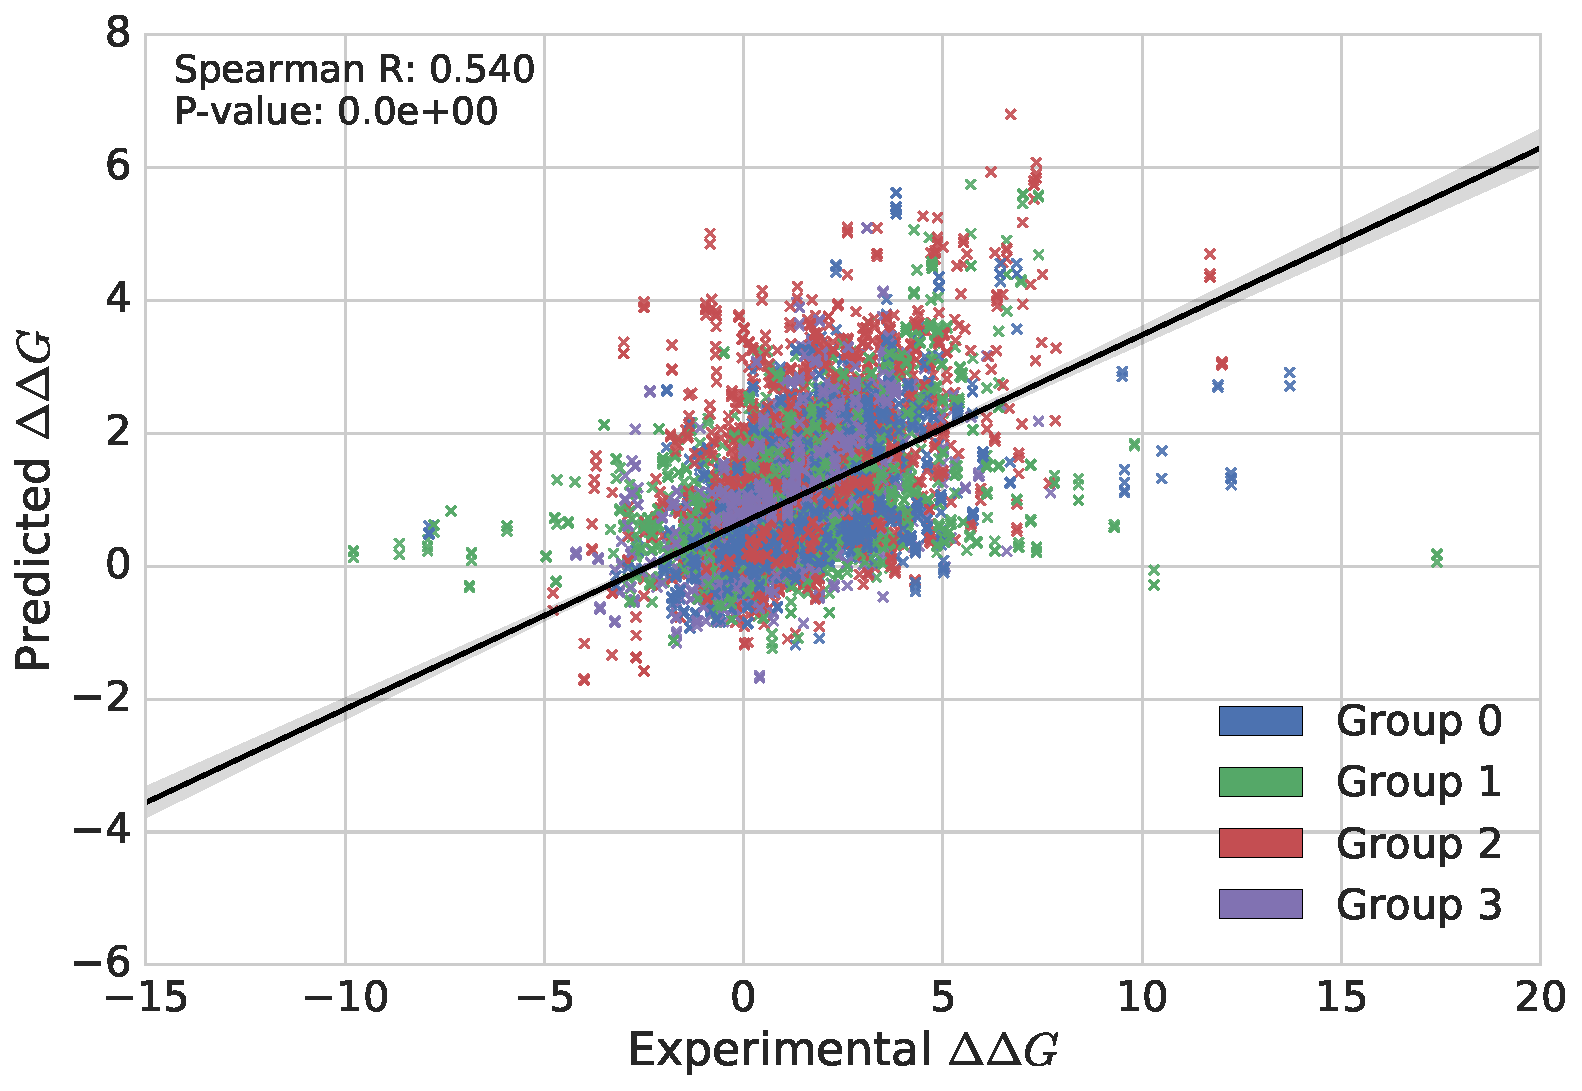
\includegraphics[width=0.6\linewidth]{static/elaspic_training_set/validation/crossvalidation_performance_core.pdf}
		\caption{Four-fold cross-validation performance on the training dataset. Colors indicate cross-validation bins.}
		\vspace*{10mm}
	\end{subfigure}
	\begin{subfigure}[b]{1.0\textwidth}
		\centering
		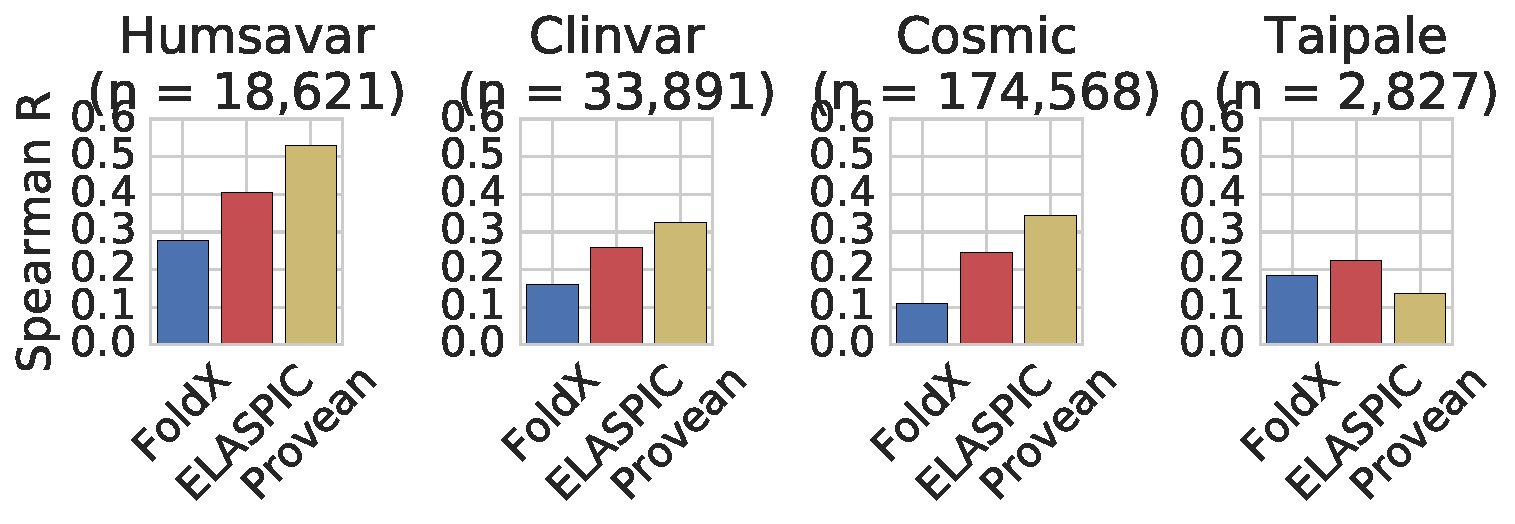
\includegraphics[width=0.8\textwidth]{static/elaspic_training_set/validation/validation_performance_core.pdf}
		\caption{Performance on the validation datasets.}
		\vspace*{10mm}
	\end{subfigure}
	\begin{subfigure}[b]{1.0\textwidth}
		\centering
		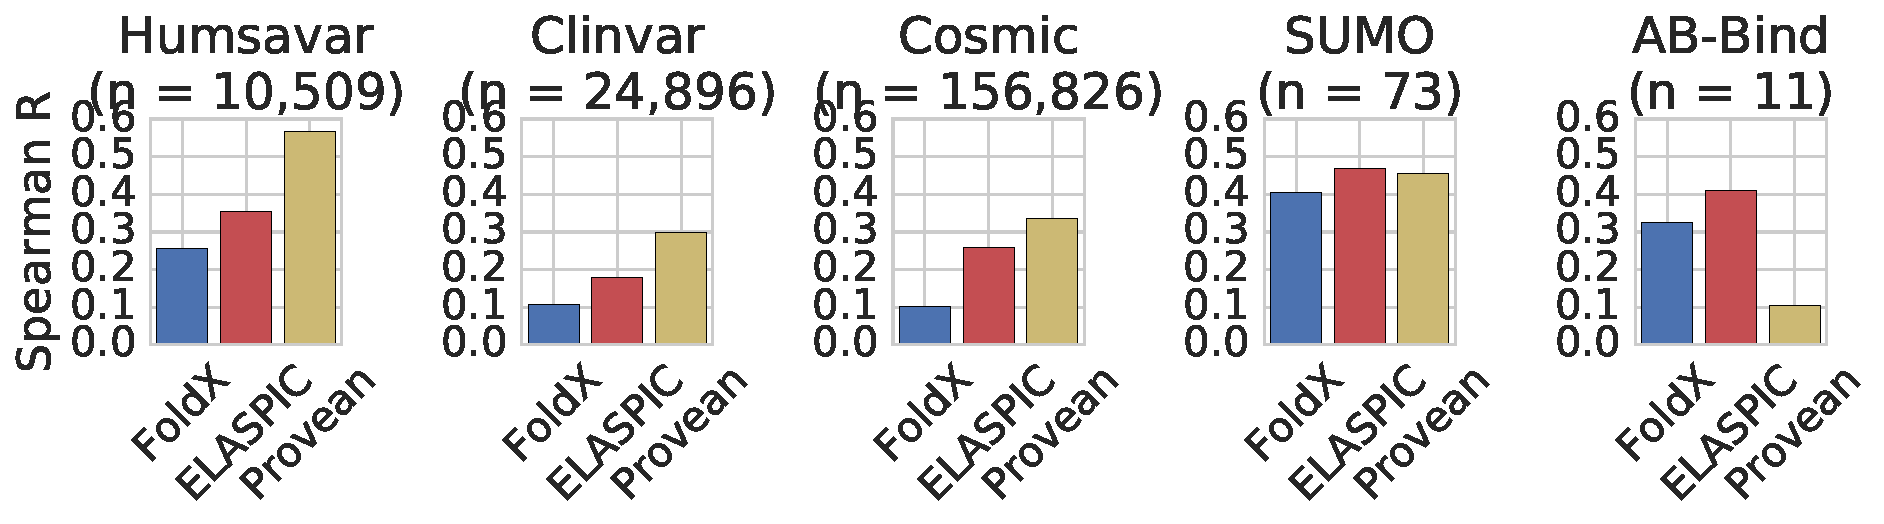
\includegraphics[width=1.0\textwidth]{static/elaspic_training_set/validation/test_performance_core.pdf}
		\caption{Performance on the test datasets.}
		% \vspace*{10mm}
	\end{subfigure}
	\caption[Core predictor validation.]{Performance of the core predictor on the training (a), validation (b) and test sets (c).}
\end{figure}



\clearpage

\section{Predicting mutation induced change in Gibbs free energy of protein-protein interactions.}

\subsection{Gridsearch and feature elimination}

\subsection{Validation}


\begin{figure}[!htb]
	\centering
	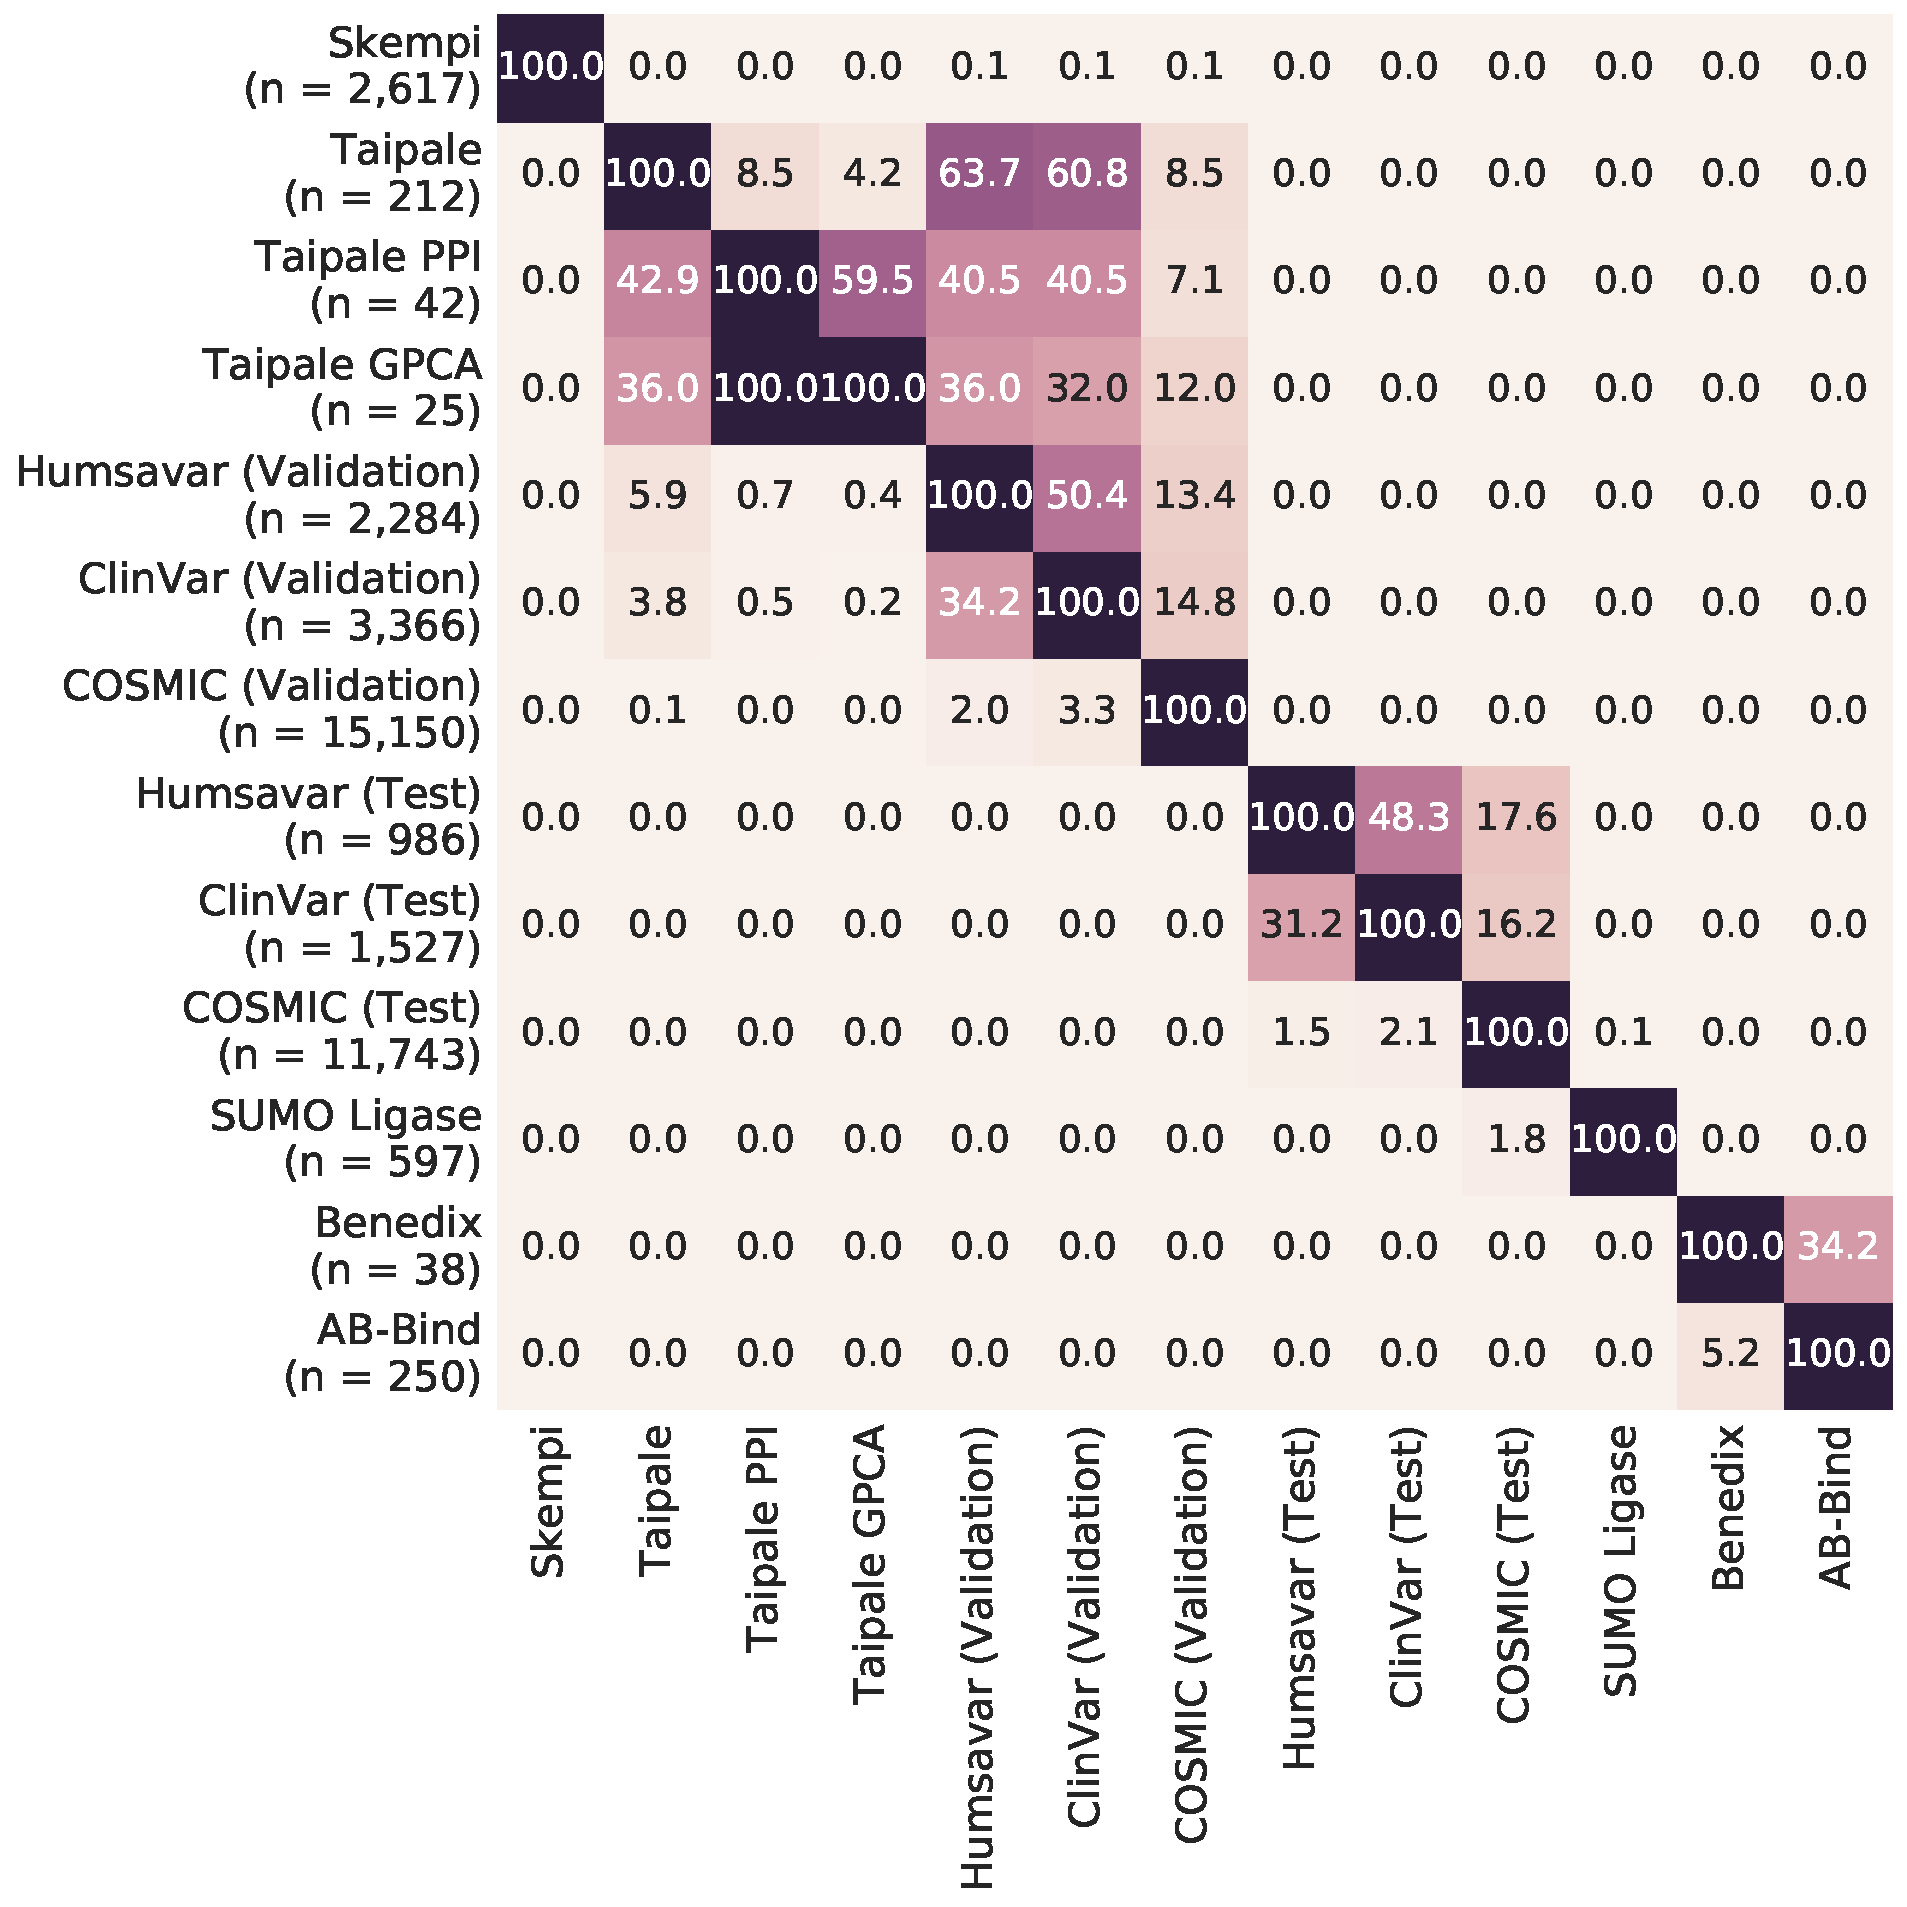
\includegraphics[width=0.9\textwidth]{static/elaspic_training_set/data_statistics/training_set_overlap_data_df_tt_interface.pdf}
	\caption[Interface predictor datasets.]{Size and overlap between the core and interface predictor datasets.}
\end{figure}


\begin{figure}[!htb]
	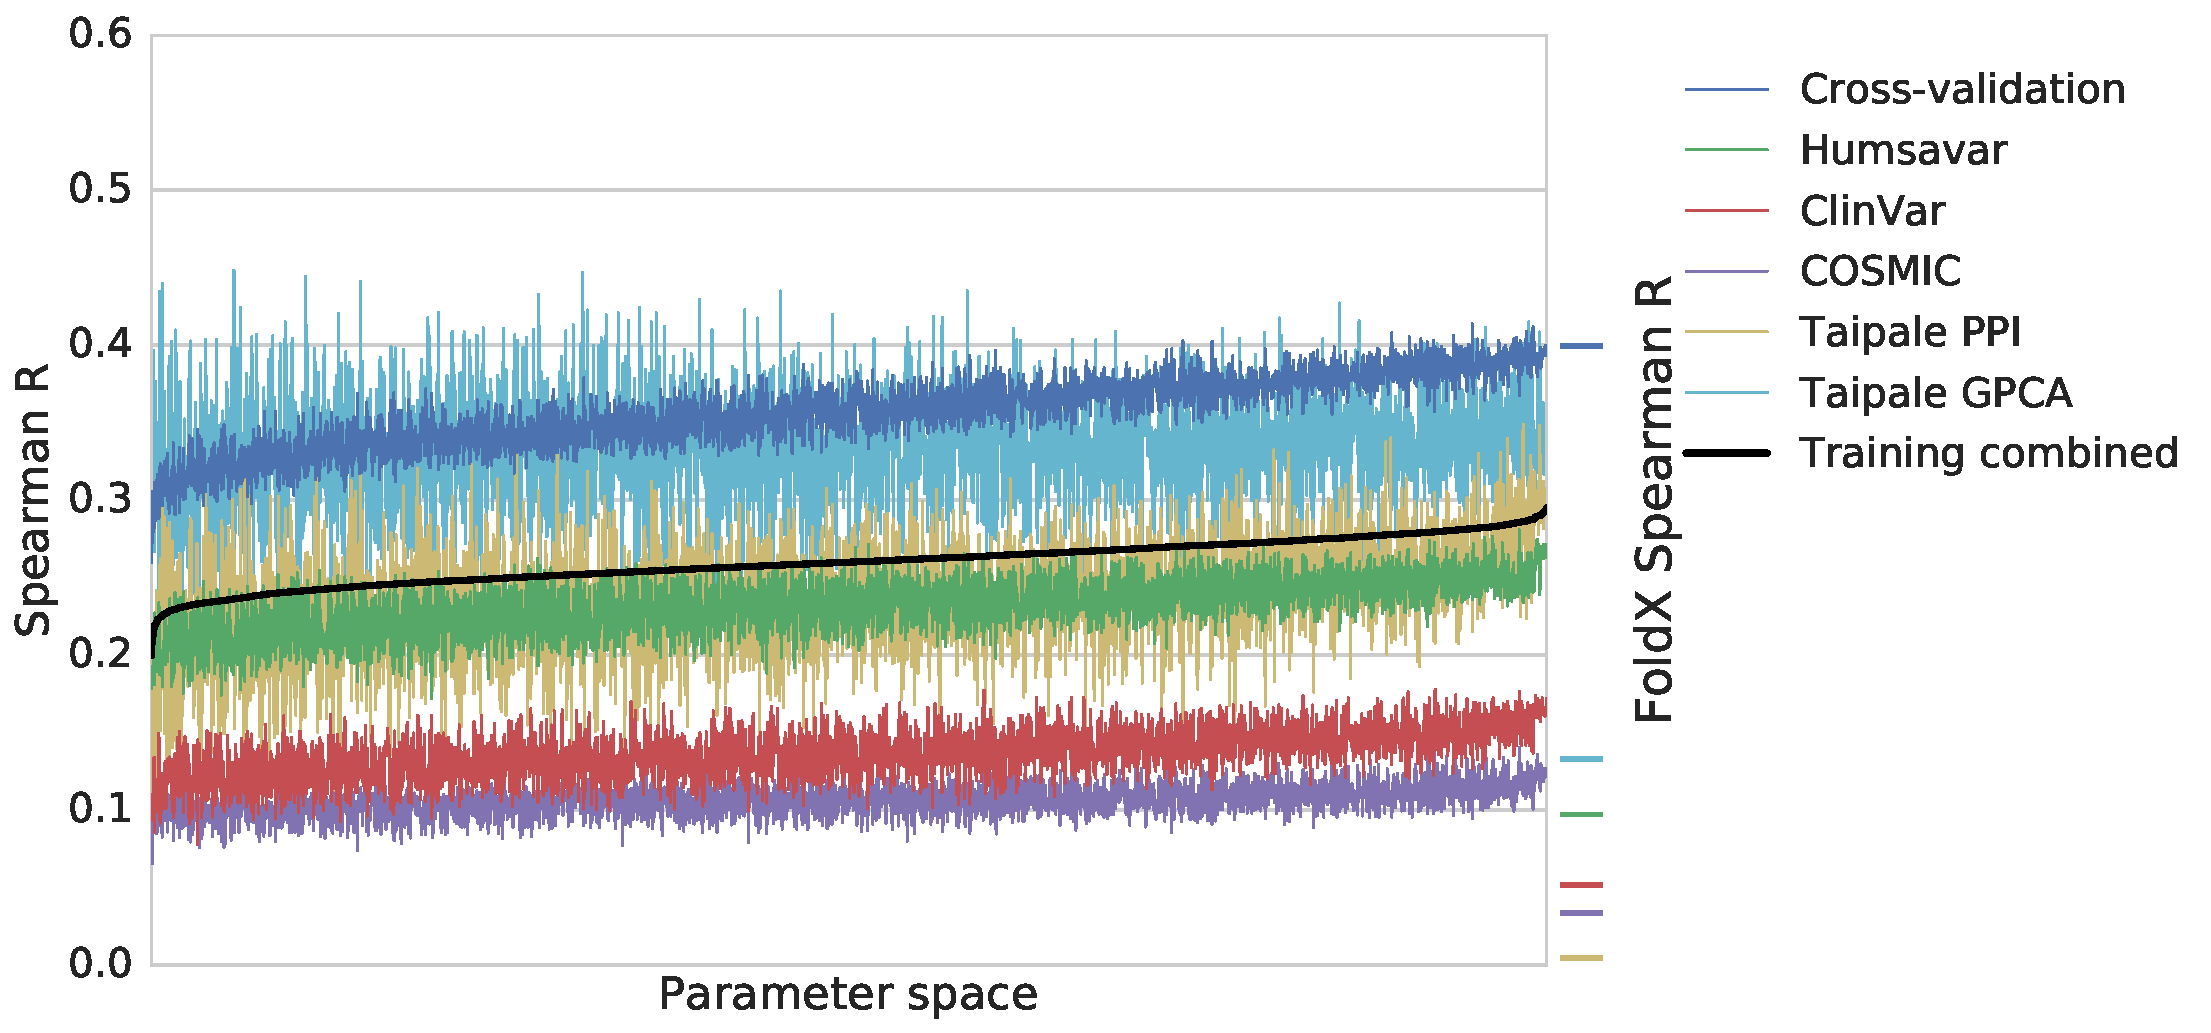
\includegraphics[width=0.9\linewidth]{static/elaspic_training_set/machine_learning/gridsearch_interface.pdf}
	\caption{Grid-search over parameter space for the ELASPIC interface predictor.}
	\label{fig:gridsearch_interface}
\end{figure}


\begin{figure}[!htb]
	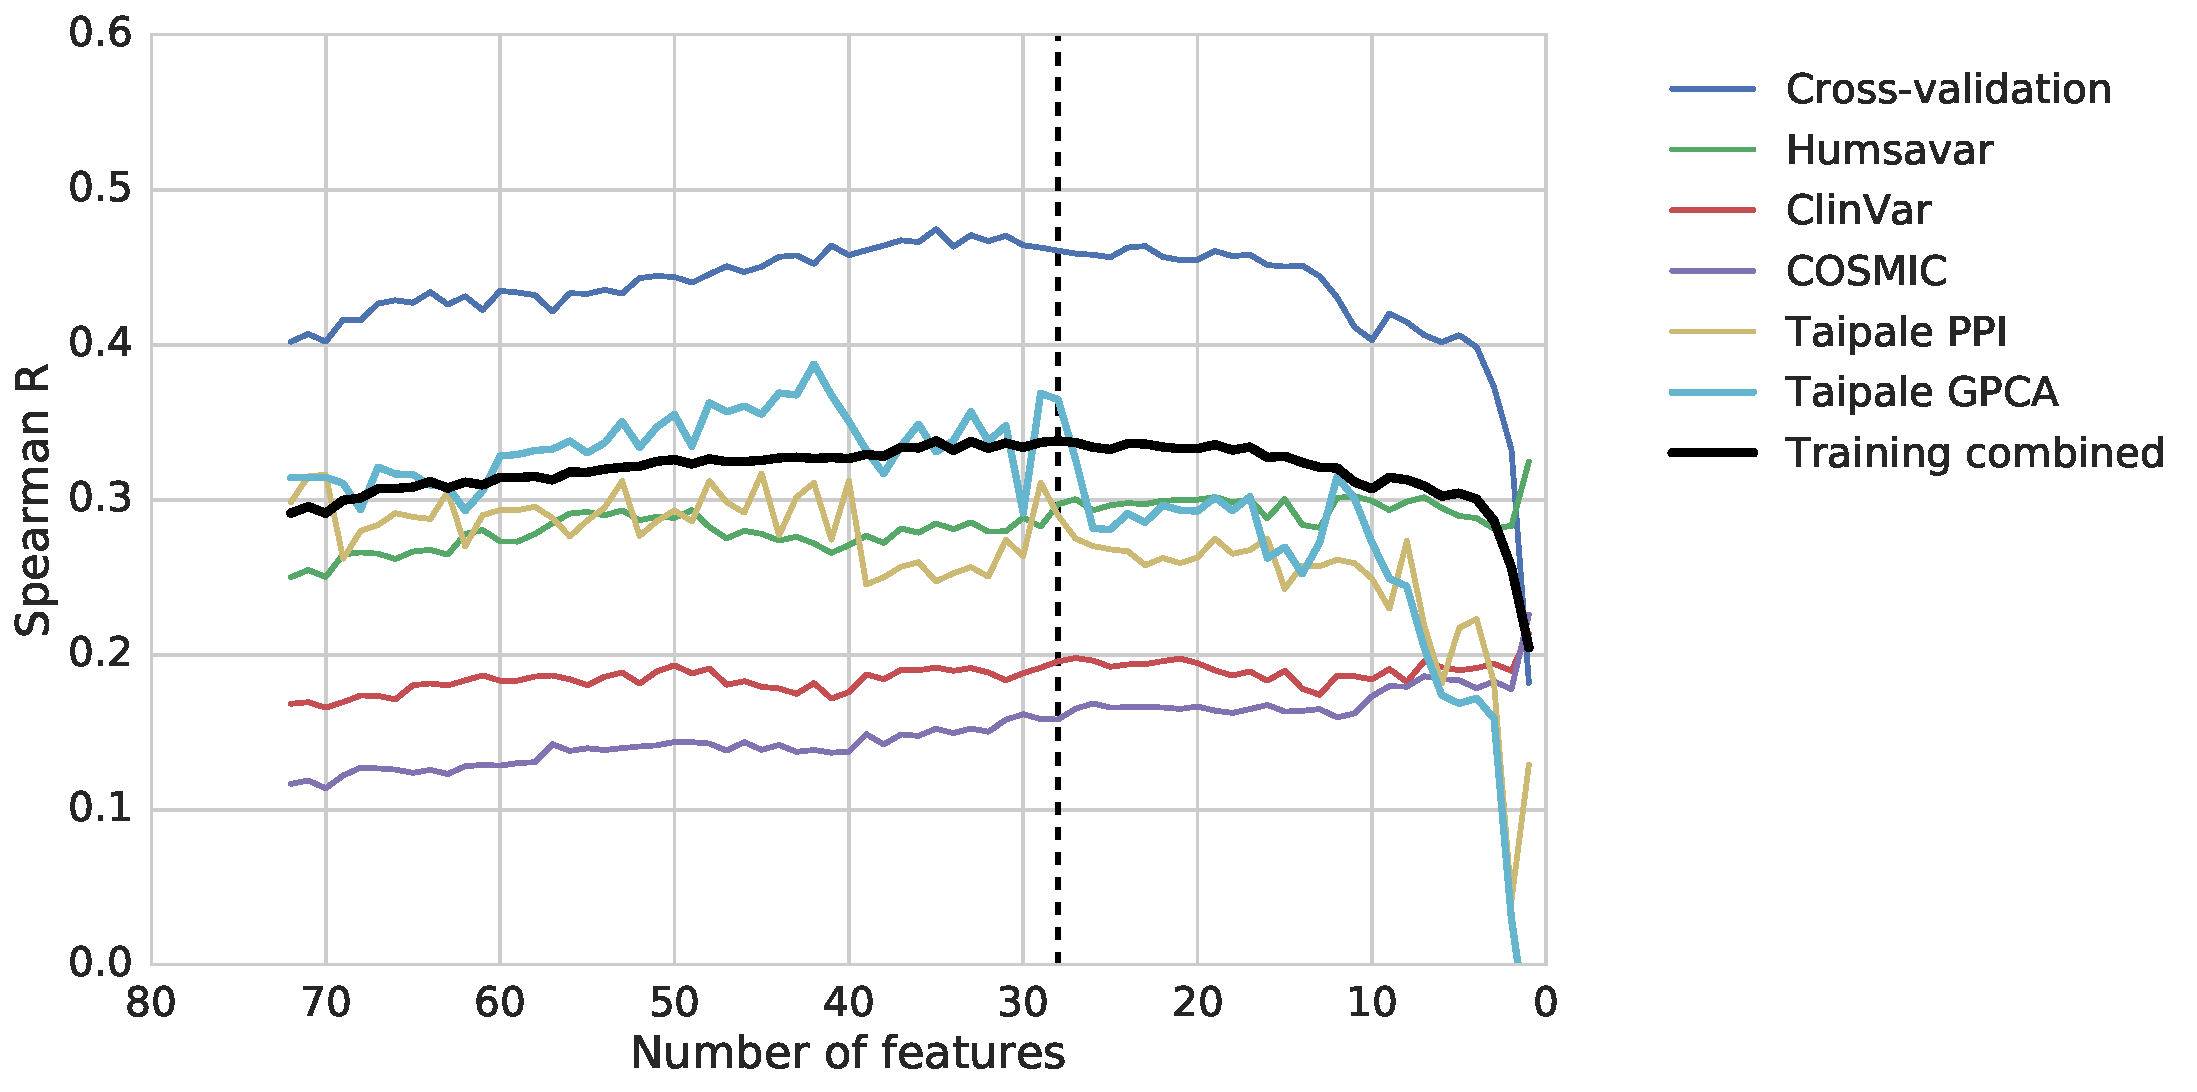
\includegraphics[width=0.9\linewidth]{static/elaspic_training_set/machine_learning/feature_elimination_interface.pdf}
	\caption{Feature elimination curve for the ELASPIC interface predictor.}
	\label{fig:feature_elimination_interface}
\end{figure}


\clearpage
\begin{table}[!htb]
	\centering
	\caption[Interface predictor parameters.]{GradientBoostingRegressor parameters selected using grid-search.}
	\label{tab:interface_parameters}
	\begin{tabular}{ l | l }
		\toprule
		Parameter name     & Parameter value \\
		\midrule
		alpha              & 0.9             \\
		learning\_rate     & 0.01            \\
		loss               & huber           \\
		max\_depth         & 4               \\
		max\_features      & 0.766           \\
		min\_samples\_leaf & 13              \\
		n\_estimators      & 2000            \\
		\bottomrule
	\end{tabular}
\end{table}


\begin{table}[!htb]
	\centering
	\caption[Interface predictor features.]{Interface predictor features. Bold indicates the top-6 most important features. FoldX feature descriptions were taken from url{http://foldxsuite.crg.eu/command/AnalyseComplex}.}
	\label{tab:interface_features}
	\begin{tabular}{ l | l | p{8cm} }
		\toprule
		Feature name                          & Feature source & Feature description                                                                                 \\
		\midrule
		alignment\_score                      & ELASPIC        & Alignment quality (Equation \ref{eq:interface_alignment_score})\par.                                \\
		backbone\_clash\_change               & FoldX          & Backbone-backbone Van der Waals energy.                                                             \\
		backbone\_clash\_wt                   & FoldX          & Backbone-backbone Van der Waals energy.                                                             \\
		backbone\_hbond\_change               & FoldX          & Backbone hydrogen bond energy.                                                                      \\
		cis\_bond\_wt                         & FoldX          & Cis peptide bond energy.                                                                            \\
		electrostatic\_kon\_wt                & FoldX          & Electrostatic interaction between molecules in the pre-complex.                                     \\
		energy\_ionisation\_wt                & FoldX          & Ionization energy.                                                                                  \\
		entropy\_complex\_change              & FoldX          & Entropic cost of forming a complex.                                                                 \\
		\textbf{entropy\_sidechain\_change}   & FoldX          & Entropic cost of fixing the side chain.                                                             \\
		intraclashes\_energy\_2\_change       & FoldX          & Van der Waals clashes of residues at the interface of the complex with their own molecule (type 2). \\
		\textbf{partial\_covalent\_bonds\_wt} & FoldX          & Interactions with bound metals.                                                                     \\
		pcv\_hbond\_self\_change              & ELASPIC        & Hydrogen-oxygen contacts involving atoms of the mutated residue and atoms of the mutated chain.     \\
		pcv\_hbond\_wt                        & ELASPIC        & Hydrogen-oxygen contacts involving atoms of the mutated residue and atoms of the interacting chain. \\
		pcv\_salt\_equal\_self\_change        & ELASPIC        & Charge repulsions involving atoms of the mutated residue and atoms of the mutated chain.            \\
		pcv\_salt\_equal\_wt                  & ELASPIC        & Charge repulsions involving atoms of the mutated residue and atoms of the interacting chain.        \\
		pcv\_salt\_opposite\_change           & ELASPIC        & Charge attractions involving atoms of the mutated residue and atoms of the interacting chain.       \\
		pcv\_salt\_opposite\_self\_change     & ELASPIC        & Charge attractions involving atoms of the mutated residue and atoms of the mutated chain.           \\
		pcv\_salt\_opposite\_self\_wt         & ELASPIC        & Charge attractions involving atoms of the mutated residue and atoms of the mutated chain.           \\
		pcv\_vdw\_self\_change                & ELASPIC        & Carbon carbon contacts involving atoms of the mutated residue and atoms of the mutated chain.       \\
		\textbf{pcv\_vdw\_self\_wt}           & ELASPIC        & Carbon carbon contacts involving atoms of the mutated residue and atoms of the mutated chain.       \\
		\textbf{pcv\_vdw\_wt}                 & ELASPIC        & Carbon carbon contacts involving atoms of the mutated residue and atoms of the interacting chain.   \\
		\textbf{provean\_score}               & Provean        & Sequence conservation score.                                                                        \\
		sloop\_entropy\_change                & FoldX          & Entropic cost according to the SLoop database of loop conformations.                                \\
		solvation\_hydrophobic\_change        & FoldX          & Contribution of hydrophobic groups.                                                                 \\
		\textbf{solvation\_polar\_change}     & FoldX          & Energetic penalty for burying polar groups.                                                         \\
		solvation\_polar\_wt                  & FoldX          & Energetic penalty for burying polar groups.                                                         \\
		torsional\_clash\_change              & FoldX          & Intra-residue Van der Waals torsional clashes.                                                      \\
		water\_bridge\_change                 & FoldX          & Contribution of water bridges.                                                                      \\
		\bottomrule
	\end{tabular}
\end{table}


\begin{figure}[!htb]
	\centering
	\begin{subfigure}[b]{1.0\textwidth}
		\centering
		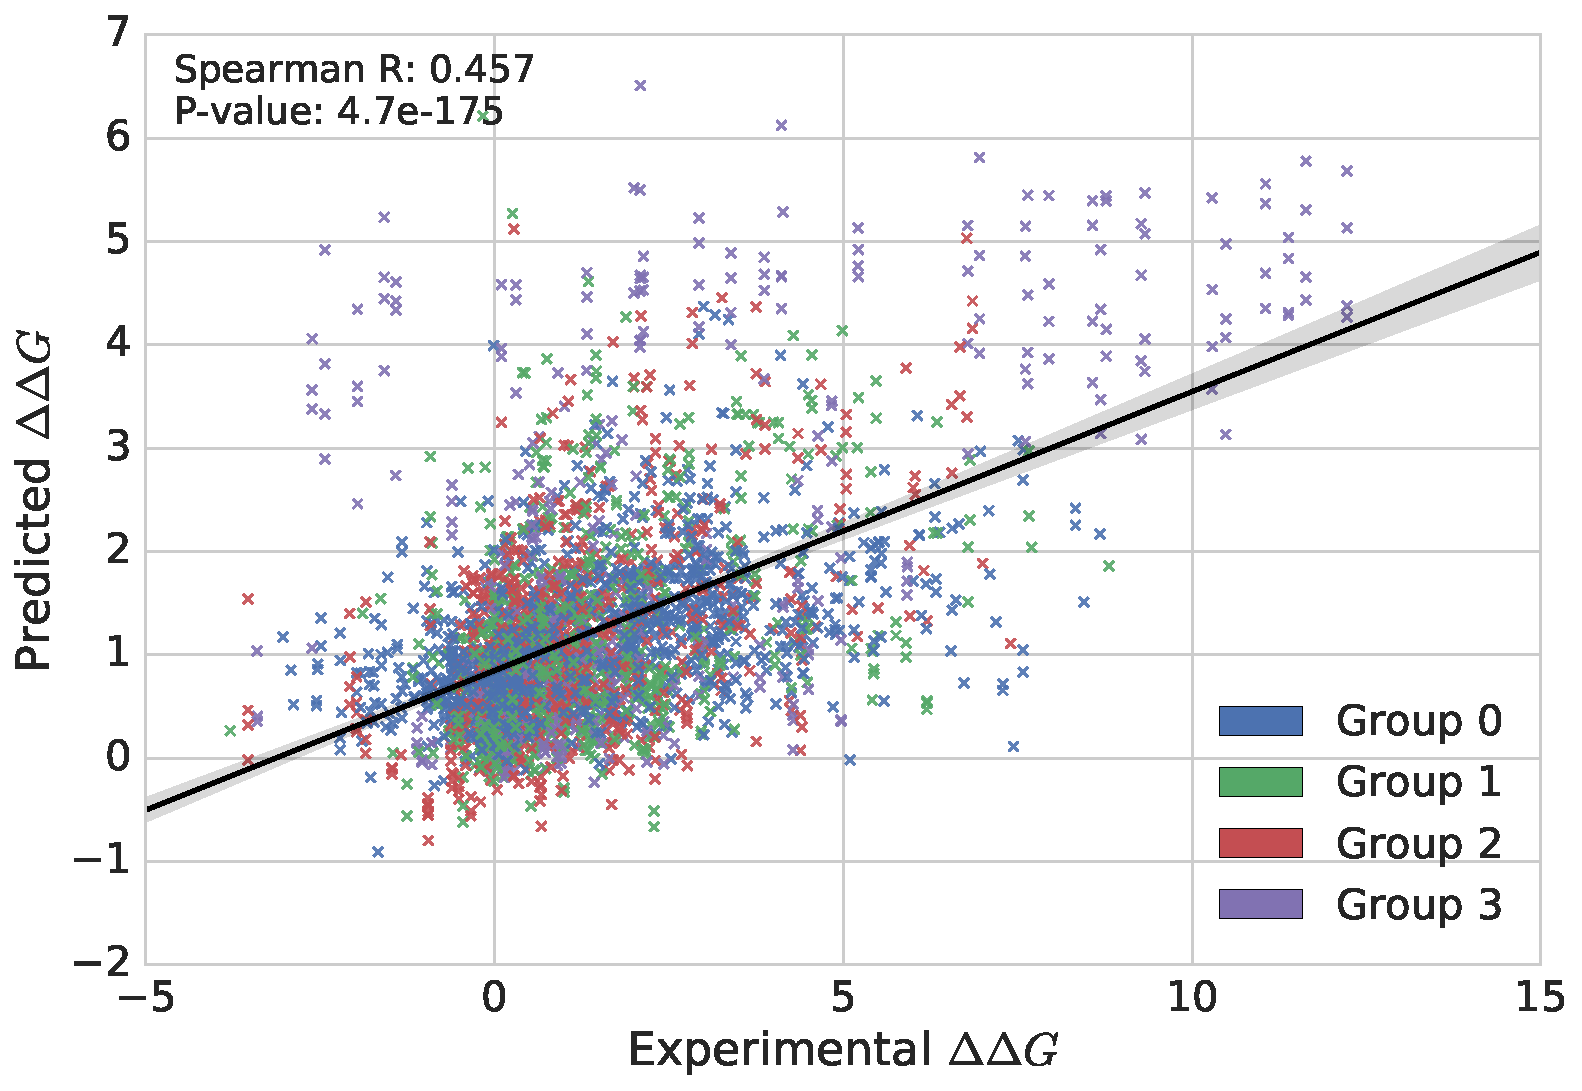
\includegraphics[width=0.6\linewidth]{static/elaspic_training_set/validation/crossvalidation_performance_interface.pdf}
		\caption{Four-fold cross-validation performance on the training dataset. Colors indicate cross-validation bins.}
		\vspace*{10mm}
	\end{subfigure}
	\begin{subfigure}[b]{1.0\textwidth}
		\centering
		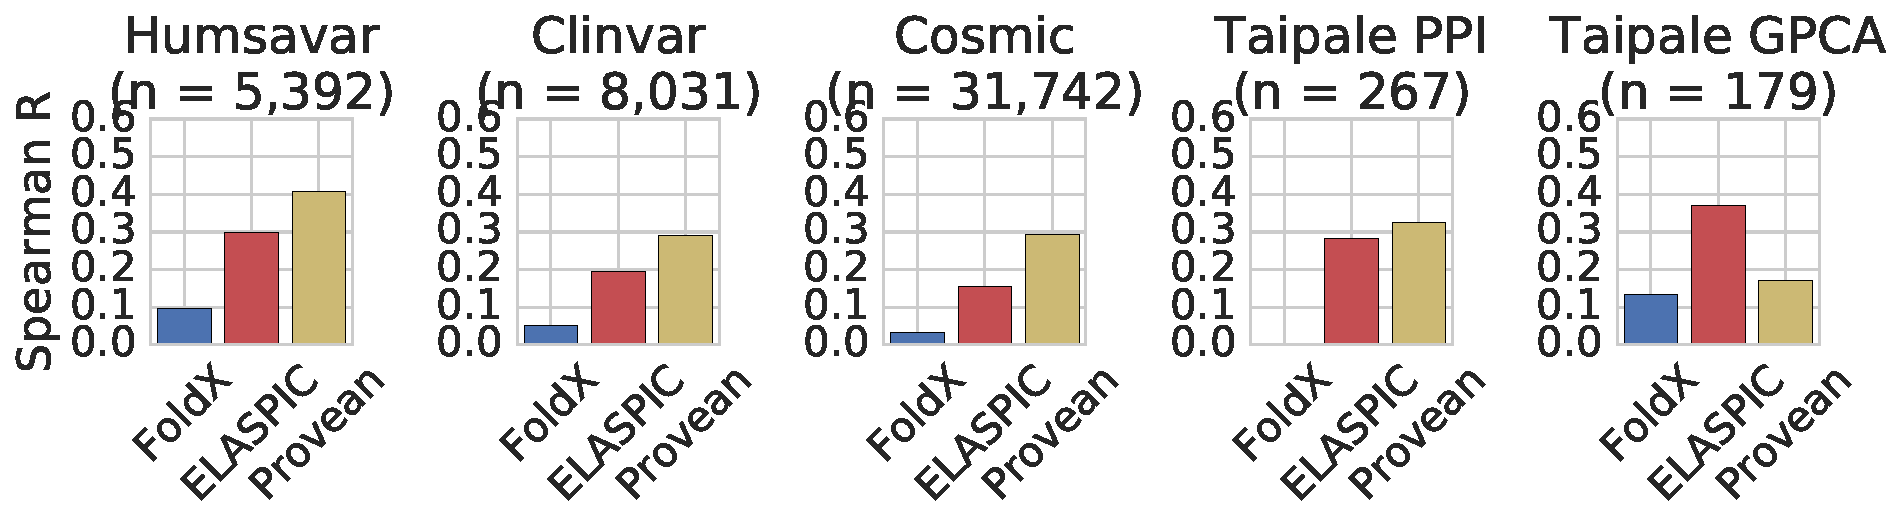
\includegraphics[width=0.9\textwidth]{static/elaspic_training_set/validation/validation_performance_interface.pdf}
		\caption{Performance on the validation datasets.}
		\vspace*{10mm}
	\end{subfigure}
	\begin{subfigure}[b]{1.0\textwidth}
		\centering
		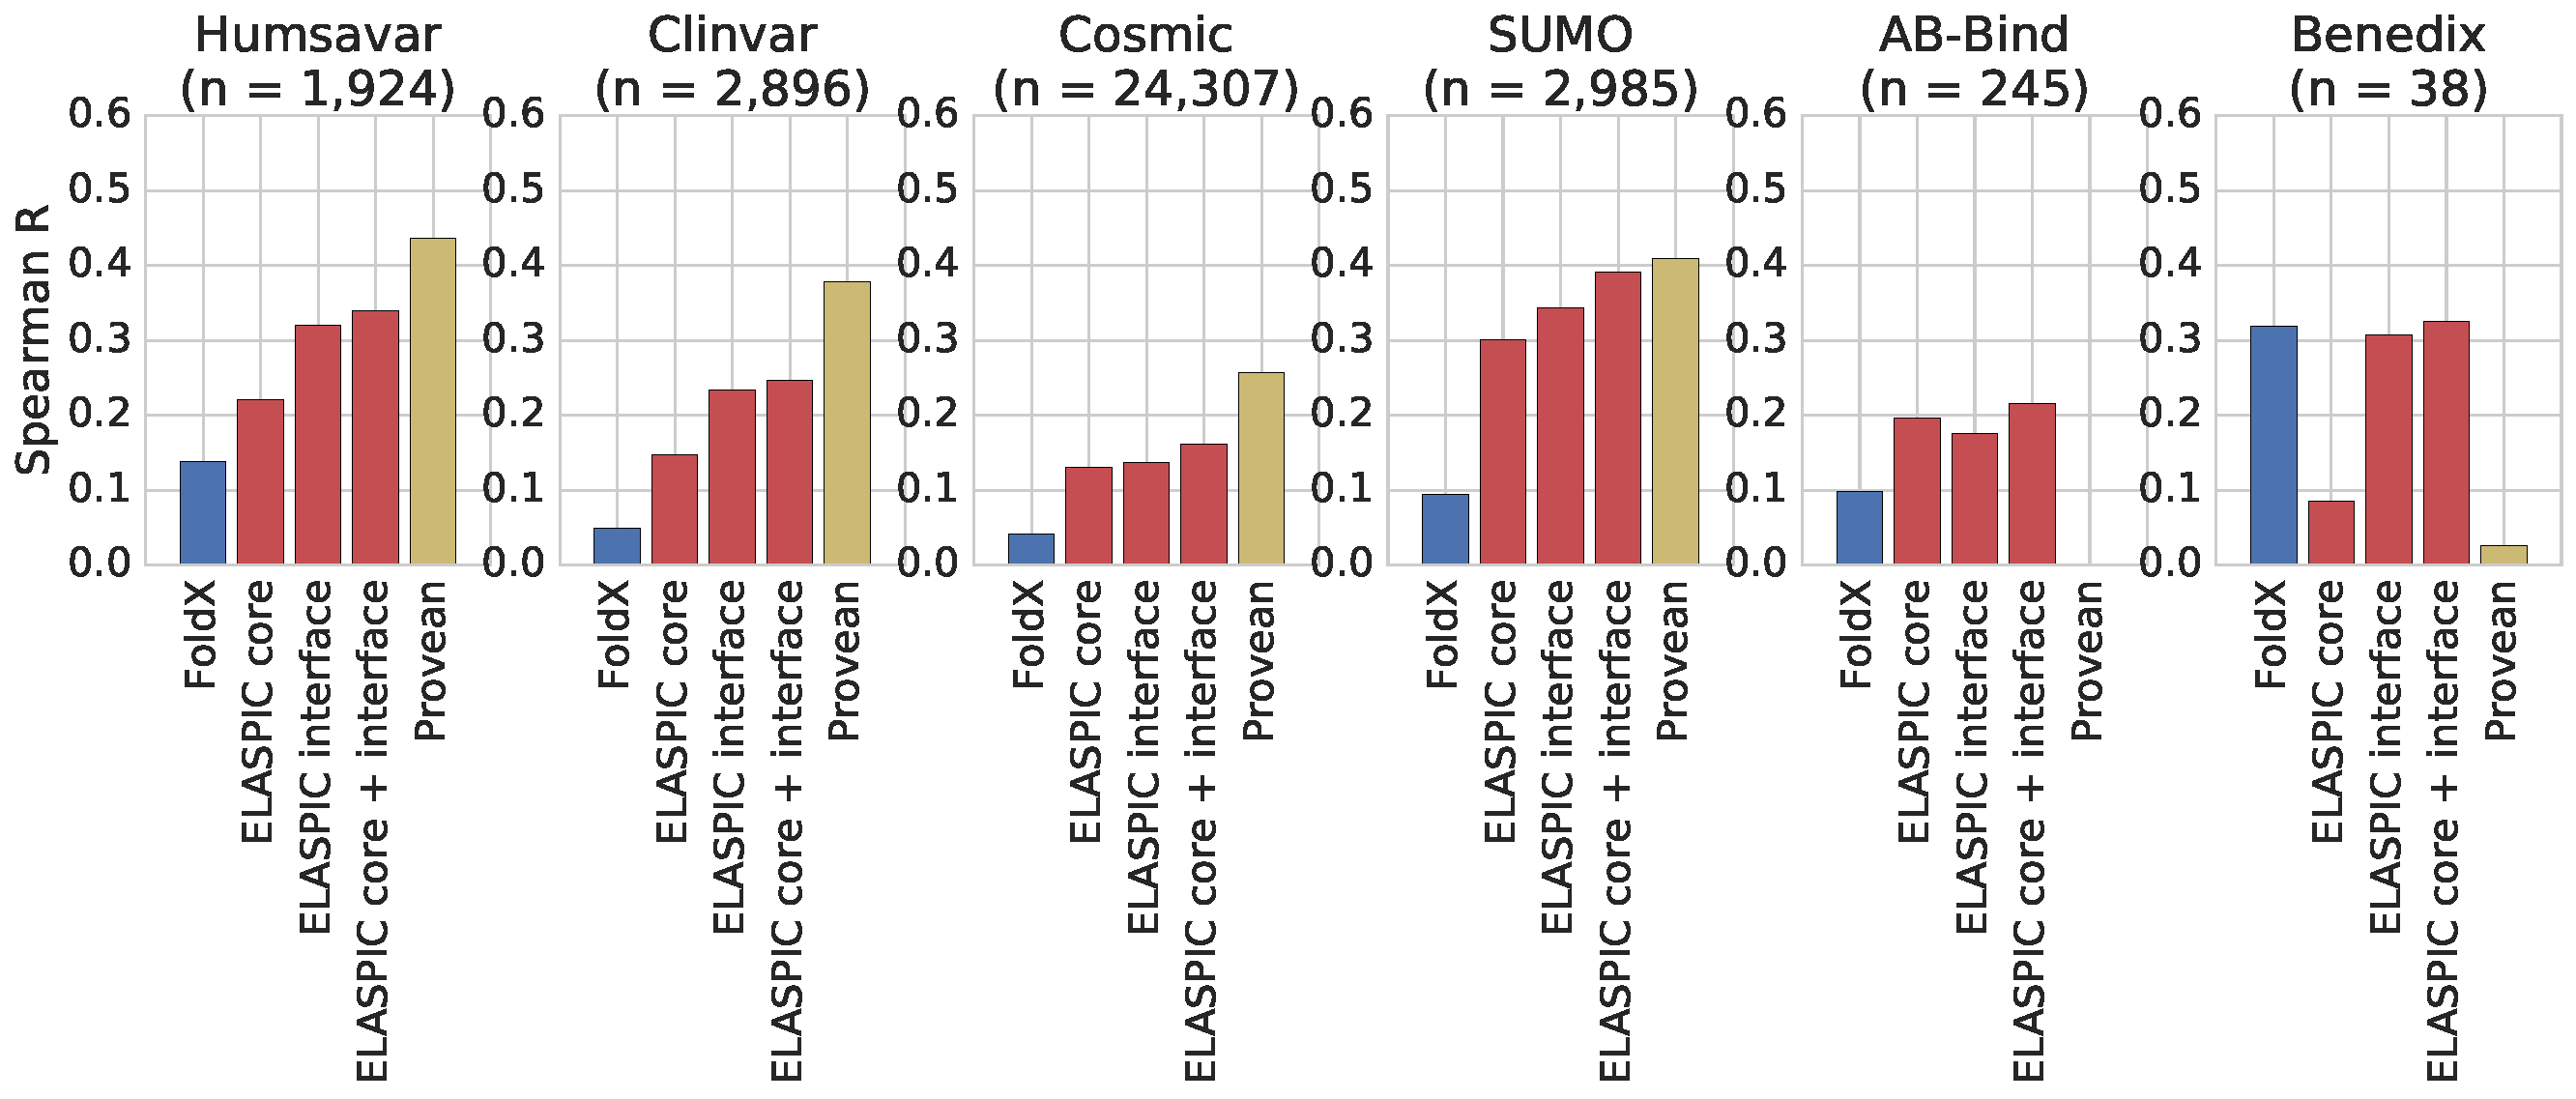
\includegraphics[width=1.0\textwidth]{static/elaspic_training_set/validation/test_performance_interface.pdf}
		\caption{Performance on the test datasets.}
		% \vspace*{10mm}
	\end{subfigure}
	\caption[Interface predictor validation.]{Performance of the interface predictor on the training (a), validation (b) and test sets (c).}
\end{figure}
